\chapter{Divergences, Propagators, and the Supersymmetric Motive}

We were supposed to begin supersymmetry proper here, but the lecture does something more careful first: it backs up and rebuilds the motivation. The real issue is not yet the algebra of supersymmetry. The real issue is the ultraviolet sensitivity of particle masses, especially scalar masses, and the way simple loop diagrams force us to confront fine tuning. Accordingly, we begin with propagators, dimensional analysis, and the simplest divergent corrections. Only then do we ask what kind of mathematical structure could make the dangerous terms cancel.

\section{Why We Are Still Talking About Divergences}

A large part of particle physics consists of calculating Feynman diagrams. They govern scattering amplitudes, of course, but that is not their only use. They also help us construct an effective Lagrangian: an approximate description in which very short-distance details have been integrated out or replaced by a cutoff.

That point is important for the present lecture. An effective Lagrangian is not merely a convenient rewrite of the exact theory. It is a controlled approximation, and the control parameter is typically a shortest distance or, equivalently, a largest momentum. From the beginning, then, the lecture is preparing us to look at the same ultraviolet difficulty in two languages:
\begin{itemize}
\item in position space, as a singularity when two points approach one another;
\item in momentum space, as a divergence from integrating over arbitrarily large momenta.
\end{itemize}

The central object in both descriptions is the propagator.

\section{Propagators in Position Space and Momentum Space}

Let us begin with the scalar field. If a particle is created at one spacetime point and detected at another, the corresponding amplitude depends only on the separation between the points. Writing
\begin{equation}
\Delta^\mu = y^\mu - x^\mu,
\end{equation}
we may think of the scalar propagator schematically as a vacuum expectation value
\begin{equation}
G_\phi(x,y) \sim \langle 0 | \phi(x)\phi(y) | 0 \rangle,
\end{equation}
with the understanding that the lecture is using this formula schematically, as an amplitude from one point to another, rather than dwelling on formal ordering subtleties.

Exactly the same diagram can also be described in momentum space. A closed loop, for example, may be viewed in either of two ways:
\begin{itemize}
\item as a propagator from a point back to itself;
\item as an integral over all momentum that can circulate around the loop.
\end{itemize}

The first viewpoint emphasizes short distances; the second emphasizes high momenta.

\subsection{Question \& Answer}

\textbf{Question.} Why are short-distance divergences and high-momentum divergences the same thing?

\textbf{Answer.} Because momentum is inverse wavelength. Large momentum corresponds to very short wavelength, and therefore to very fine spatial resolution. So a singularity at \(\Delta \to 0\) in position space is the same ultraviolet phenomenon as a divergence from integrating over very large loop momentum in momentum space. The lecture insists on this equivalence early, because every later estimate can be read in either language.

\section{Scalar Fields, Dimensional Analysis, and the Massless Propagator}

The lecture next narrows to scalar particles. A scalar field has one component, and in four dimensions its simplest action may be written schematically as
\begin{equation}
S_\phi \sim \int d^4x\, (\partial_\mu \phi)^2.
\end{equation}
The exact normalization and metric-signature conventions are not the point here. What matters is dimensional analysis.

In the units used throughout the lecture, \(\hbar=c=1\), so the action is dimensionless. Since \(d^4x\) contributes four powers of length and each derivative contributes one inverse power of length, we have
\begin{align}
1 &\sim [S_\phi] \sim [d^4x]\,[\partial_\mu \phi]^2 \\
  &\sim L^4 \left(L^{-1}[\phi]\right)^2.
\end{align}
It follows immediately that
\begin{equation}
[\phi] = L^{-1}.
\end{equation}

Now add the familiar mass term and quartic interaction:
\begin{equation}
S_\phi \sim \int d^4x \left[(\partial_\mu\phi)^2 - m^2\phi^2 - \lambda \phi^4\right].
\end{equation}
Again suppressing inessential numerical factors, dimensional consistency gives
\begin{equation}
[m]=L^{-1}, \qquad [\lambda]=L^0.
\end{equation}
So the quartic scalar coupling is dimensionless in four spacetime dimensions.

Once we know the dimension of \(\phi\), the short-distance form of the massless propagator is essentially forced on us. Translation invariance says that it depends only on \(x-y\), Lorentz invariance says that it depends only on the invariant interval, and dimensional analysis says that the answer must carry the dimensions of two scalar fields. Therefore
\begin{equation}
G_\phi(\Delta) \propto \frac{1}{\Delta^2},
\qquad
\Delta^2 = \Delta_\mu \Delta^\mu.
\end{equation}
There are numerical constants here, but not new scales.

A nonzero mass changes the propagator at large distance, not at very short distance. The lecture makes this vivid with the relativistic dispersion relation:
\begin{equation}
E=\sqrt{p^2+m^2},
\qquad
E=|p|
\quad \text{for a massless particle.}
\end{equation}
When \(|p|\gg m\), the massive expression forgets the mass and approaches the massless one. That is the ultraviolet lesson: short-distance propagation is dominated by very large momentum, and very large momentum is insensitive to the mass.

For large separations one expects a suppression of the schematic form
\begin{equation}
G_{\phi,m}(\Delta) \approx \frac{1}{\Delta^2}\, e^{-m\Delta},
\end{equation}
where the exponential should be understood as a mnemonic for the large-distance cutoff introduced by the mass. Near \(\Delta=0\), however, the factor \(e^{-m\Delta}\) is approximately \(1\), and the singular behavior remains \(1/\Delta^2\).

\section{The Simplest Scalar Self-Energy Diagram and the Fine-Tuning Problem}

At this point the lecture turns from general propagator lore to the first genuinely dangerous diagram: the simplest scalar loop correction. The blackboard at this moment still carries part of the earlier discussion of dimensions and relativistic kinematics, while the central diagram has already changed into a loop correction.

\begin{figure}[t]
\centering

\includegraphics[width=0.82\textwidth]{lecture_03_figure_02.png}
\caption{Simple loop correction with surrounding field-theory formulas. The board still retains the nearby kinematic relation \(E=\sqrt{p^2+m^2}\), its massless limit \(E=|p|\), and part of the scalar-field dimensional analysis while the discussion turns to the simplest loop correction.}
\end{figure}

The surrounding formulas visible on the board are exactly the ones that motivate the transition:
\begin{equation}
E=\sqrt{p^2+m^2},
\qquad
E=|p|,
\qquad
[\phi]=L^{-1}.
\end{equation}
So the loop diagram is not appearing in isolation. It is appearing at the end of a chain of reasoning about short distances, dimensions, and the fact that masses are irrelevant in the ultraviolet.

\begin{figure}[t]
\centering
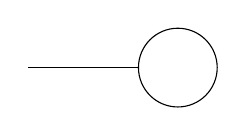
\begin{tikzpicture}[scale=1.0]
\draw (-2.0,0) -- (-0.6,0);
\draw (-0.1,0) circle (0.5);
\end{tikzpicture}
\caption{Schematic redraw of the simplest scalar self-energy correction. The exact vertex geometry on the board is not fully sharp, so the redraw is kept minimal.}
\end{figure}

The lecture interprets this diagram as a correction to the scalar mass term. In a \(\lambda\phi^4\) theory, its size is of order
\begin{equation}
\delta m_\phi^2 \sim \lambda\, G_\phi(0).
\end{equation}
But \(G_\phi(\Delta)\sim 1/\Delta^2\), so at coincident points the propagator is singular. If we admit that our field theory should not be trusted below some shortest distance \(\delta\), then we replace the coincident-point singularity by the cutoff estimate
\begin{equation}
\delta m_\phi^2 \sim \frac{\lambda}{\delta^2}.
\end{equation}
This is the quadratic divergence.

\subsection{Question \& Answer}

\textbf{Question.} Why does this simplest scalar loop correction behave like \(\lambda/\delta^2\)?

\textbf{Answer.} Because the diagram is just a quartic vertex weighted by \(\lambda\), multiplied by the scalar propagator from a point back to itself. The short-distance form of that propagator is \(1/\Delta^2\). At coincidence this diverges, and with a shortest-distance cutoff \(\delta\) the only available estimate is \(1/\delta^2\). No delicate calculation is needed to see the scaling.

This is the point at which the lecture brings the Higgs boson into focus. A scalar mass that is supposed to be small compared with the cutoff receives a correction that naturally wants to be of order \(1/\delta^2\). One can certainly tune the bare mass against this loop correction, but that is exactly the fine-tuning problem. In momentum space the same statement is that too much ultraviolet momentum can circulate in the loop. In position space it is the singularity of the propagator at very small separation. They are the same problem.

\section{Fermions: Dirac Fields and Short-Distance Propagation}

Only after the scalar problem has been made sharp does the lecture turn to fermions. The structure is parallel, but not identical. The Dirac action is written schematically as
\begin{equation}
S_\psi \sim \int d^4x\, \bar\psi\,\gamma^\mu \partial_\mu \psi
\end{equation}
with a mass term of the form
\begin{equation}
\int d^4x\, m\,\bar\psi\psi.
\end{equation}
The gamma matrices are dimensionless, and there is only one derivative. Therefore
\begin{align}
1 &\sim [S_\psi]
   \sim [d^4x]\,[\bar\psi]\,[\partial_\mu]\,[\psi] \\
  &\sim L^4 [\psi]^2 L^{-1}.
\end{align}
So
\begin{equation}
[\psi] = L^{-3/2}.
\end{equation}
The lecture pauses over the half-integer power, but this is exactly the expected fermionic pattern: half-integers keep appearing.

It is then easy to check that the fermion mass really has the dimension of mass:
\begin{equation}
[d^4x]\,[m]\,[\bar\psi\psi]
\sim L^4 \cdot L^{-1} \cdot L^{-3} \sim 1.
\end{equation}

Now repeat the scalar argument for the short-distance propagator. Since the propagator carries the dimensions of two fermion fields, its massless form must scale as
\begin{equation}
S_\psi(\Delta) \sim \frac{1}{\Delta^3}.
\end{equation}
If we restore the spinor structure that the lecture temporarily suppresses, then one inserts a gamma matrix and one factor of the separation vector upstairs:
\begin{equation}
S_{ij}(\Delta) \propto \frac{(\gamma_\mu \Delta^\mu)_{ij}}{\Delta^4}.
\end{equation}
That refined form will not be needed for the crude ultraviolet estimates, but it explains why the dimensional shorthand \(1/\Delta^3\) is correct.

Just as in the scalar case, a nonzero fermion mass modifies the propagator at large separations but does not change the leading short-distance behavior.

\section{Closed Fermion Loops, Yukawa Couplings, and the Supersymmetric Motive}

We are now ready to ask the question the lecture has really been aiming toward: can a fermionic loop cancel the dangerous scalar self-energy correction?

There are two separate issues:
\begin{itemize}
\item the sign of a closed fermion loop;
\item the size of the ultraviolet divergence in a scalar--fermion loop.
\end{itemize}

\subsection{Question \& Answer}

\textbf{Question.} Why does a closed fermion loop carry the opposite sign from a closed boson loop?

\textbf{Answer.} The lecture gives a very pretty exchange argument. Start with two identical disconnected loops. Their product is positive regardless of the sign of each single-loop factor. Now cut and reconnect by exchanging the particles. For bosons, exchanging identical particles produces no minus sign because the two-particle wavefunction is symmetric:
\begin{equation}
\Psi_B(x_1,x_2)=+\Psi_B(x_2,x_1).
\end{equation}
For fermions, exchanging identical particles produces a minus sign because the wavefunction is antisymmetric:
\begin{equation}
\Psi_F(x_1,x_2)=-\Psi_F(x_2,x_1).
\end{equation}
But after the exchange, the reconnected object is just a one-loop diagram. Therefore the one-loop fermion diagram has the opposite sign from the one-loop boson diagram. In this lecture that sign is the crucial opening through which cancellation may become possible.

The next step is to estimate a fermion loop coupled to the scalar through a Yukawa interaction,
\begin{equation}
g\,\phi\,\bar\psi\psi.
\end{equation}
Its coupling is dimensionless, as one sees immediately from
\begin{align}
1 &\sim [d^4x]\,[g]\,[\phi]\,[\bar\psi\psi] \\
  &\sim L^4 \,[g]\, L^{-1}\,L^{-3}.
\end{align}
Hence
\begin{equation}
[g]=L^0.
\end{equation}

Now estimate the loop itself. There are two Yukawa vertices, contributing \(g^2\), and two fermion propagators, each contributing \(1/\Delta^3\). Holding one point fixed and integrating over the separation of the other point, we get
\begin{equation}
\mathcal{A}_f \sim -g^2 \int d^4\Delta\, \frac{1}{\Delta^6}.
\end{equation}
The minus sign is the closed-fermion-loop sign just discussed. Dimensional analysis then gives
\begin{equation}
\mathcal{A}_f \sim -\frac{g^2}{\delta^2}.
\end{equation}
So the fermion loop has exactly the same degree of divergence as the bosonic scalar loop, but with the opposite sign.

This is the payoff of the lecture. The scalar loop wants to give
\begin{equation}
+\frac{\lambda}{\delta^2},
\end{equation}
while the fermionic Yukawa loop wants to give
\begin{equation}
-\frac{g^2}{\delta^2}.
\end{equation}
At last there is a mechanism that can threaten the quadratic divergence. But it is not enough merely to have a minus sign. One would need the couplings to match in the right way,
\begin{equation}
g^2 \sim \lambda,
\end{equation}
and for exact cancellation one would also want the bosonic and fermionic masses to match closely enough that their propagators agree in the ultraviolet. If the masses are unequal, the full cancellation is incomplete; nevertheless, the leading divergent piece can still cancel provided the short-distance behavior remains sufficiently similar.

And now the lecture reaches the threshold of supersymmetry without yet entering the formal theory. It would be an extraordinary accident if nature chose all these relations by hand. What one wants is a mathematical structure that enforces them. That is the motive for supersymmetry: not a decorative extension of the Standard Model, but a symmetry principle powerful enough to relate bosons and fermions so that the dangerous scalar divergences are tamed.

\section{Summary}

The lecture deliberately postpones the formal machinery of supersymmetry and instead reconstructs the problem that makes such a symmetry desirable. We begin with propagators, see why short distances and high momenta are the same ultraviolet regime, derive the scalar and fermion propagators by dimensional analysis, and then compare their simplest loop corrections. The scalar self-energy is quadratically divergent; a fermion loop can produce the same divergence with the opposite sign. That is the opening. Supersymmetry enters as the candidate structure that can turn this opening into a systematic cancellation by tying together couplings and masses rather than leaving them to numerical accident.